\section{Araxis Merge}
\paragraph{}
This piece of software is able to perform pixel by pixel comparison of two input images. It can be used to display the differences between them. See image \ref{fig:araxis_input_output} to become familiar with its abilities.

\begin{figure}[H]
     \centering
     \subfloat[]{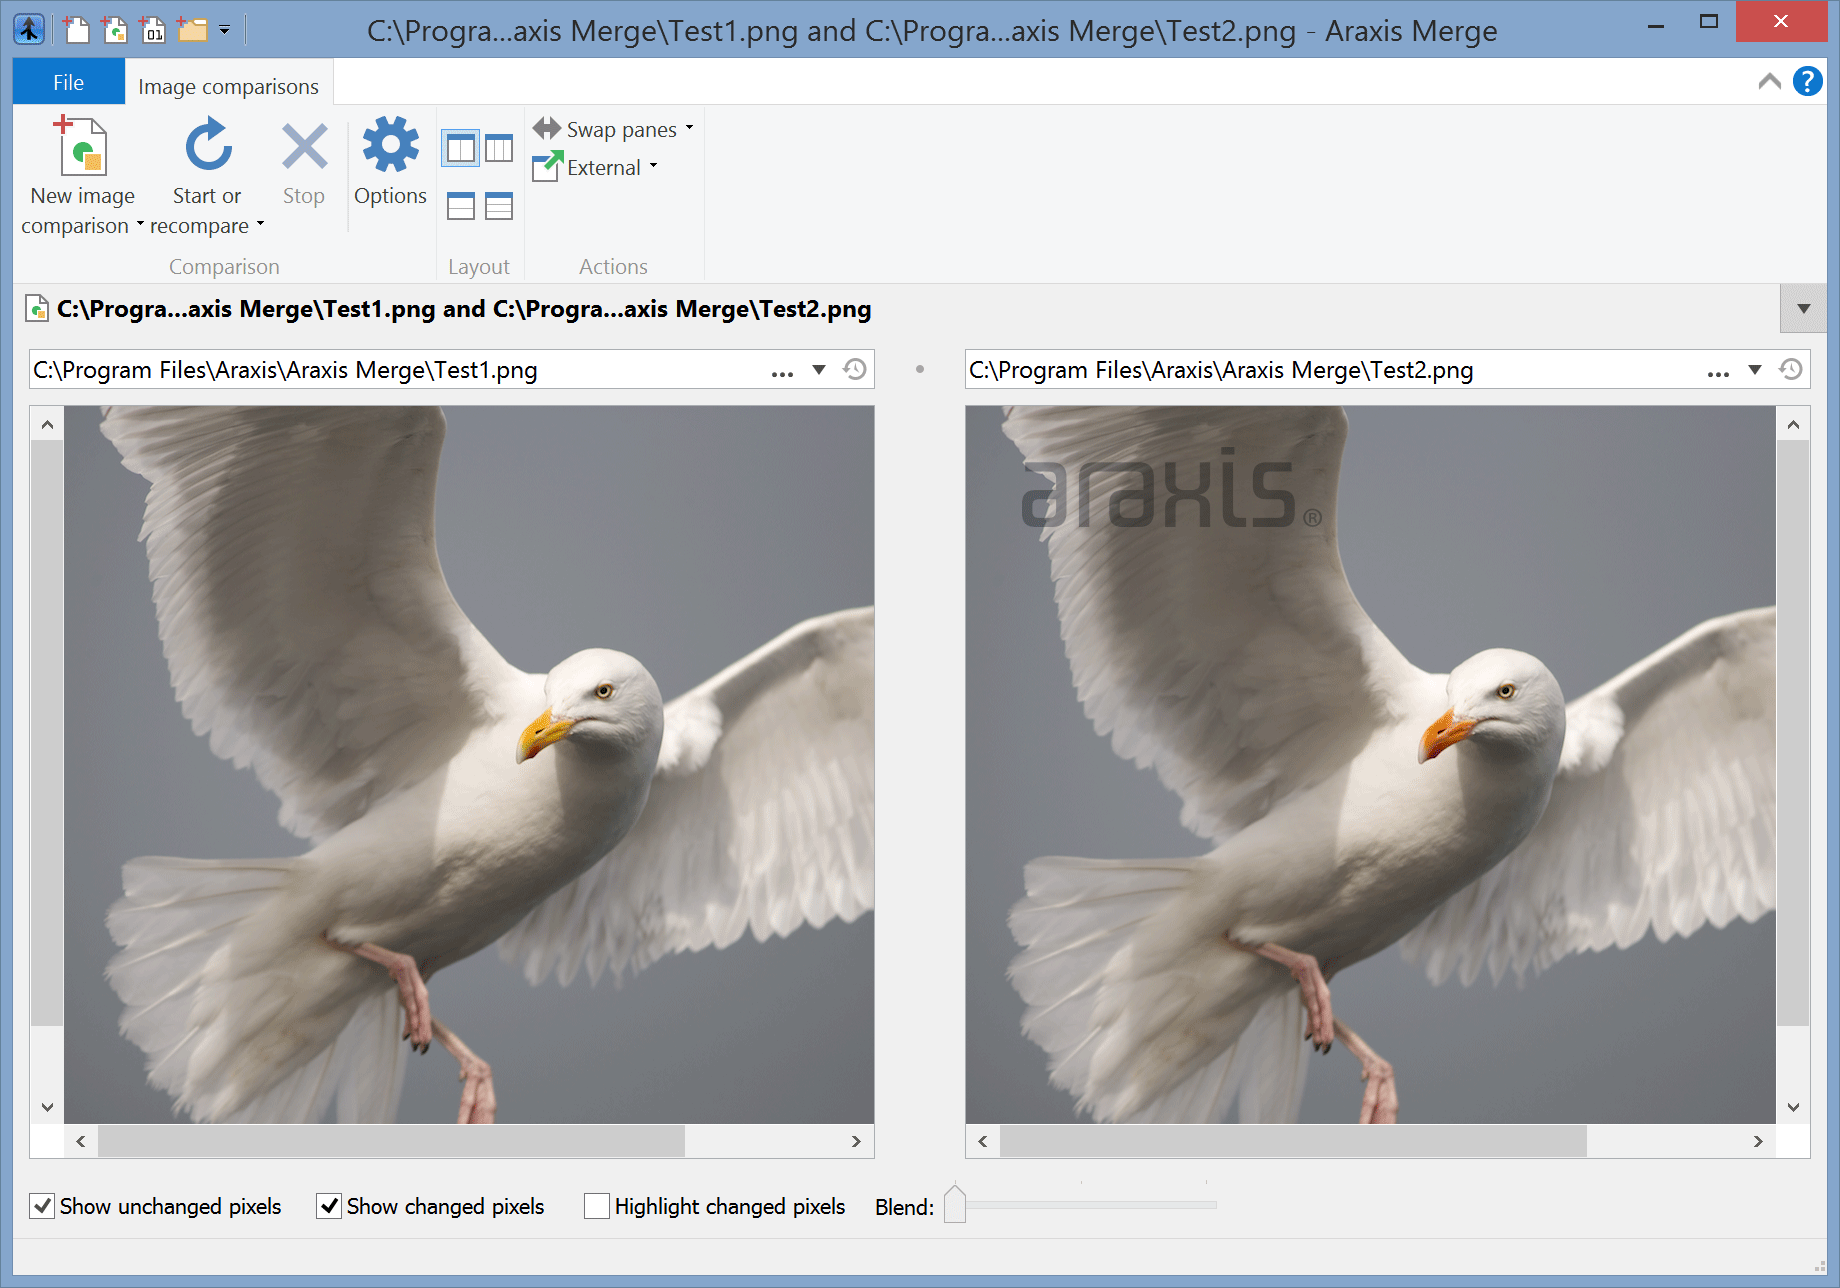
\includegraphics[width=0.45\textwidth]{images/araxis_1}}
     \qquad
     \subfloat[]{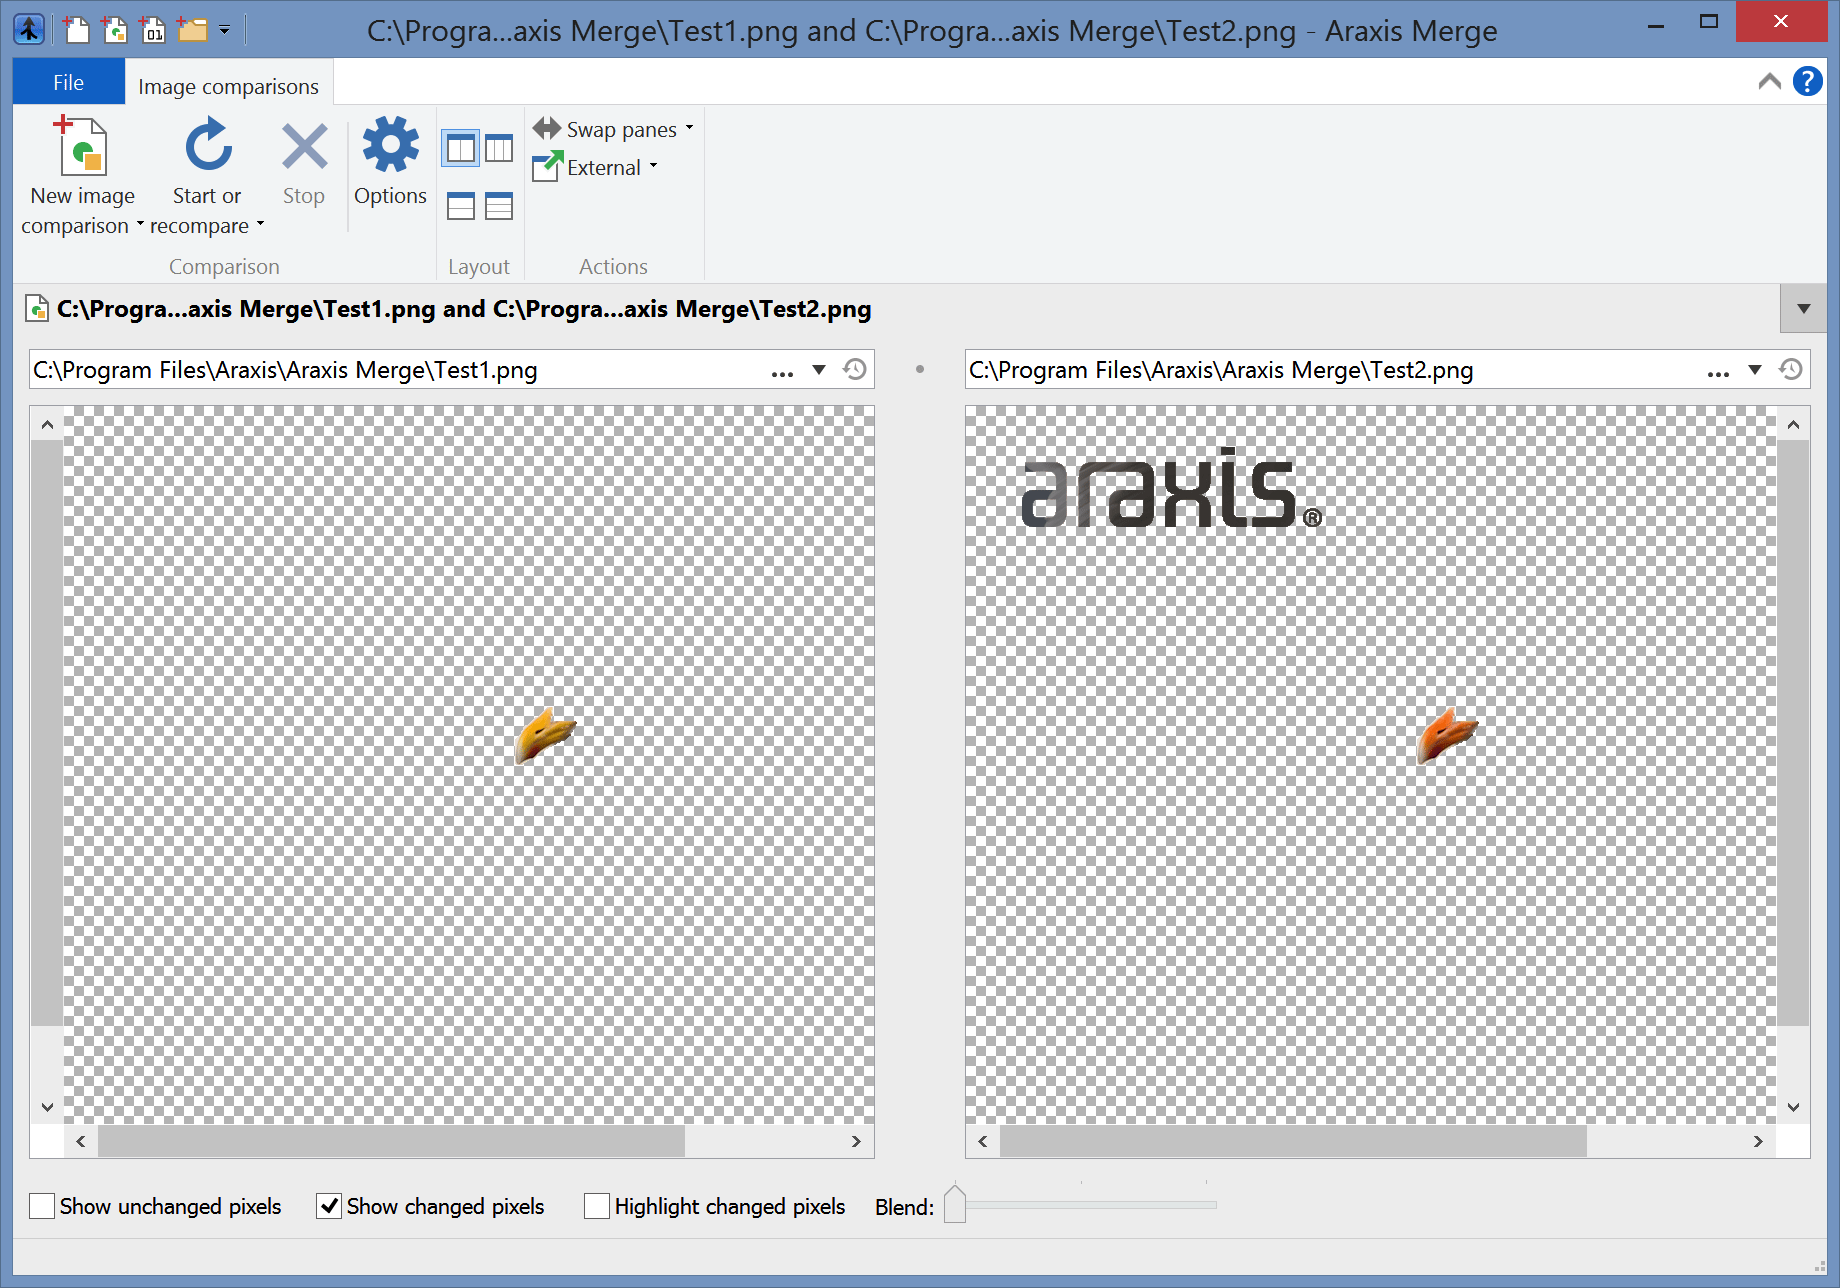
\includegraphics[width=0.45\textwidth]{images/araxis_2}}
     \caption{Araxis Merge example}
     \source{\url{https://www.araxis.com/merge/documentation-windows/comparing-image-files}}
     \label{fig:araxis_input_output}
\end{figure}

\section{Image Comparer}
\paragraph{}
Let us now look at another available alternative. Unlike the Araxis Merge, Image Comparer analyzes and recognizes an image's content (this technology is known as content based image search), and groups pictures that look alike. Image \ref{fig:image_comparator} presents its' abilities.

\begin{figure}[h]
	\centering
	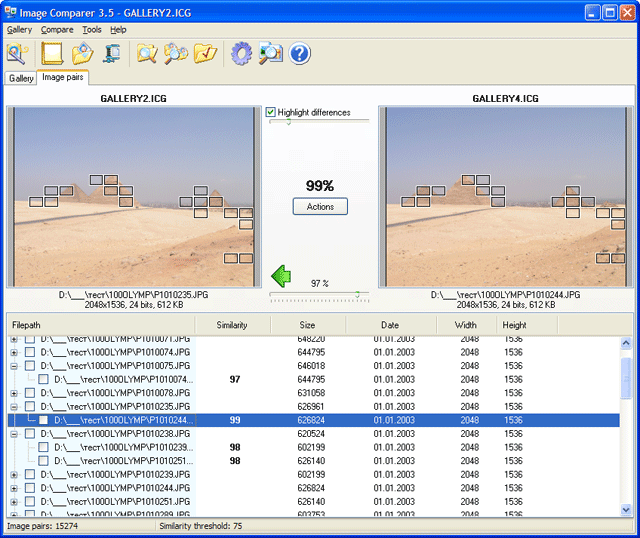
\includegraphics[width=0.6\textwidth]{images/image_comparer}
	\caption{Image Comparer example}
	\source{\url{https://www.bolidesoft.com/imagecomparer.html}}
	\label{fig:image_comparator}
\end{figure}


\section{Conclusion}
\paragraph{}
Although there exists some software for comparing images, it is mostly pixel by pixel based. Moreover, the shape of rails is the same and the interesting difference lies in the pattern on their surface. This is a very specialized task that needs to be performed.

\paragraph{}
The analysis of the state of the art has thus shown, there is no available software, which supports the identification of steel rails, that meets our requirements.